\section{Arkitektur}

\subsection{UpdateCaseRepo}

\begin{figure}[H]
    \makebox[\textwidth][c]{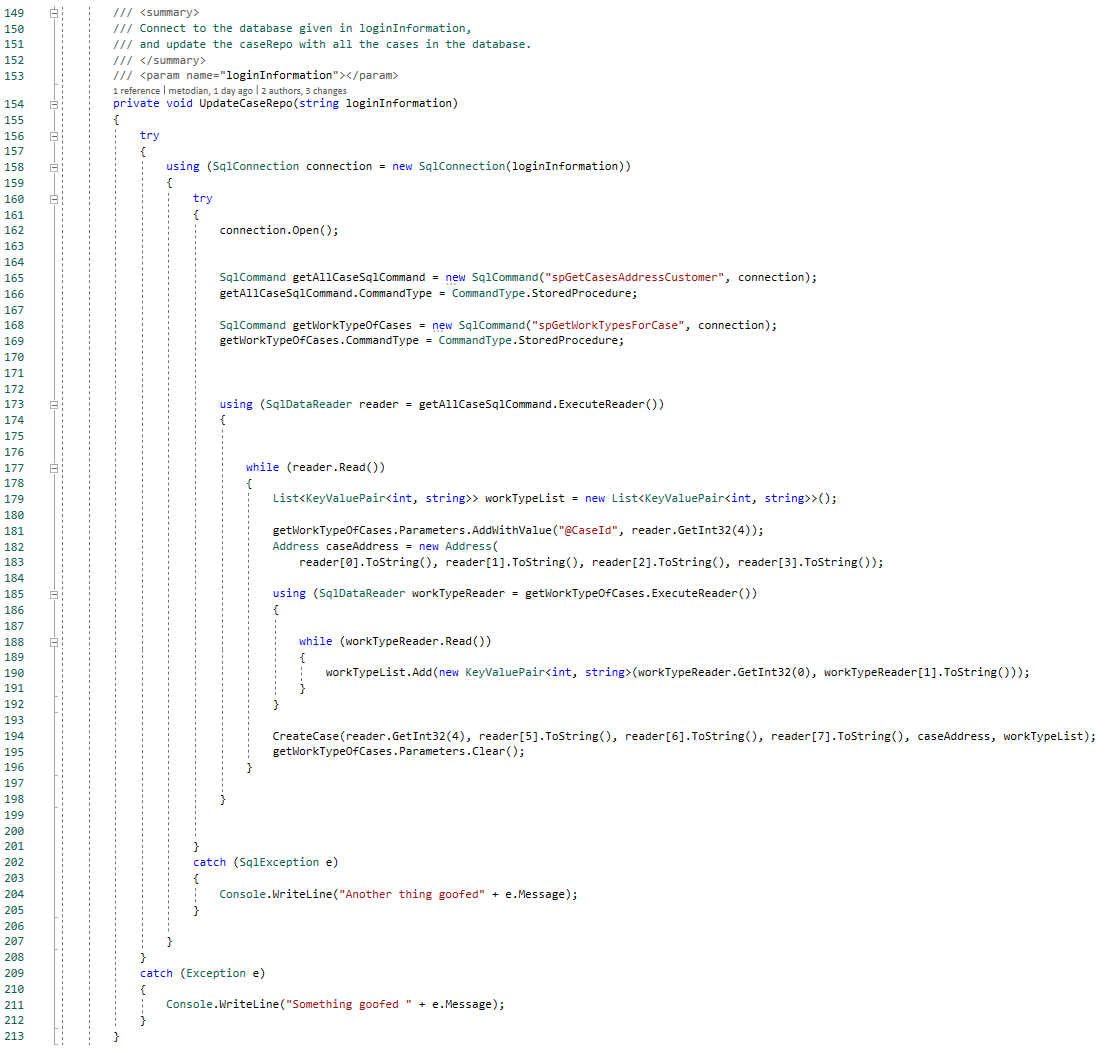
\includegraphics[scale = 0.9]{UpdateCaseRepo.PNG}}
    \caption{Her vises metoden UpdateCaseRepo, som ligger i classen CaseRepo. Denne metoder henter alle cases med til hørende customers og addresses fra databasen.}
    \label{fig:UpdateCaseRepo}
\end{figure}

I figur \ref{fig:UpdateCaseRepo} ser vi opdaterings metode som sørger for at hente alle vores cases fra databasen. UpdateCaseRepo tager som parameret en string og denne string indeholder login informationer til den database vi bruger, dette kan ses på linje 154.
Det første vi gør er at vi bruger en try og catch på Sqlconnection, for at se om vi kan lave en connection med den string metoden bruger. Hvis den ikke kan lave en Sqlconnection fanger catchen den exeception der blive smidt ud. I linje 158 bruges der keyworded using, som sørger at lukke Sqlconnection igen efter den er færdig med at bruge den, ellers skal metoden Close() bruges for at lukke forbindelen.



Efter forbindelsen er blevet åbnet med metoden Open() i linje 162, bliver der lavet to Sqlcommands (getAllCasesSqlcommand og getWorkTypeOfCases) fra linje 165 til 169. Som bliver defineret som stored procedures.[ref storedprocedures]



I linje 173 bliver der brugt en ny using hvor der bliver oprettet og eksekveret en SqlDataReader på Sqlcommanden getAllCasesSqlcommand. Efterfølgende bruges der et while loop som kører hele readeren igennem, med metoden Read() dette sker i linje 177. Hver gang reader.Read() bliver kørt bliver der indlæst en række fra databasen ind i reader. Denne reader opfører sig ligesom et Array. Inde i dette while loop på linje 179 bliver der oprettet en ny liste workTypeList, som er af typen KeyValuePair. En list af typen KeyValuePair bruges når man gerne vil associere en nøgle med en værdi. Dette gør det nemmer at finde ting i listen hvis vi ved hvad nøglen er.


Før den næste Sqlcommand getWorkTypeOfCases kan blive kørt skal der oprettets en ny parameter som sker på linje 181, denne parameret kommer fra SqlDataReader reader på plads 5, hvis du bare tager index nummert i readeren er den ikke type specifik, da vi skal bruge en interger er vi derfor nødtil at bruge metoden GetInt32() for at specificere det.


Fra linje 181 til 183 bliver der instansers et nyt address objekt, som får værdier fra SqlDataReader reader fra index 0 til og med index 4.


Efter dette bliver da lavet en ny SqlDataReader som kommer hedder workTypeReader, men før at vi kan eksekvere to readers i samme connection skal vi tilføje en ekstra parameter til vores loginInformation string på linje 154, som er \textit{MultipleActiveResultSets=True}. Inde i denne her reader bliver der oprettet og tilføjet nye KeyValuePairs til listen på linje 179.

Til sidste før at loopet bliver kørt igen bliver der oprettet et nyt case objeckt, men de resterende outputs fra getWorkTypeOfCases og det nye objekt caseAddress på linje 182 og den listen der er blevet oprettet med SqlDataReader workTypeReader.
For at kunne blive ved at bruge de samme parametre er man nød til at bruge metoden Clear() til sidste for ellers kan der ikke blive oprette en ny parameter med samme navn da den allerede eksistere.
